\documentclass[border = 5pt, tikz]{standalone}
\usepackage{xcolor, soul}
\sethlcolor{yellow}
\begin{document}
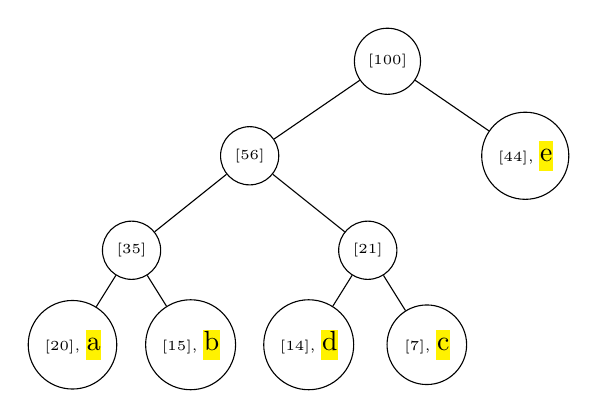
\begin{tikzpicture}[
  every node/.style = {minimum width = 2em, draw, circle},
  level 1/.style = {sibling distance = 35mm, level distance = 12mm},
  level 2/.style = {sibling distance = 30mm, level distance = 12mm},
  level 3/.style = {sibling distance = 15mm, level distance = 12mm}
  ]
  %first tree
  \node {\tiny[100]}
  child {node {\tiny[56]}
        child {node {\tiny[35]}
                child {node {\tiny [20], \normalsize \hl{a}}}
                child {node {\tiny [15], \normalsize \hl{b}}}
        }
        child {node {\tiny [21]}
                child {node {\tiny [14], \normalsize \hl{d}}}
                child {node {\tiny [7], \normalsize \hl{c}}}
        }
  }
  child {node {\tiny [44], \normalsize \hl{e}}
    };
\end{tikzpicture}
\end{document}
